% ===========================================================================
\section{Introducción}

Los motores OCR a baja resolución producen texto degradado con errores sistemáticos de
carácter: palabras partidas, caracteres mal reconocidos y secuencias numéricas corruptas. Un
trabajo propio previo ---\emph{LLM-Guided Sequence Reconstruction} (LLM-GSR)\footnote{A.\
Jaime, \emph{LLM-Guided Sequence Reconstruction for Degraded OCR Output: Closing the Latency
Gap with Parallel Inference}.}--- reconstruye esa salida tratándola como un problema de
predicción de secuencia con un LLM, y cierra la brecha de latencia paralelizando sobre
\textbf{Ray} (patrón \emph{Pure Dispatcher}). Ese trabajo resuelve la \emph{calidad} y la
\emph{velocidad}, pero no la \emph{resiliencia}: qué pasa cuando un nodo cae a mitad de una
factura, o cuando el modelo, en vez de reconstruir, \emph{inventa}.

Este trabajo agrega esa capa. La idea que lo guía es simple y fuerte: \textbf{que un sistema
distribuido procese cada factura \emph{exactamente una vez} no garantiza que el resultado sea
correcto}. Un worker puede completar su tarea \emph{limpiamente} ---sin caída ni
reintento--- y aun así entregar un resultado incorrecto: si el \textbf{modelo} que ejecuta
alucina un importe en lugar de reconstruirlo, nada en la capa de ejecución lo nota y el
sistema lo da por bueno. Por eso medimos dos problemas por separado: la \emph{pérdida de trabajo por
caídas} y la \emph{corrupción silenciosa del contenido}. Un verificador determinista
---\textbf{VERA}--- actúa como compuerta: decide qué facturas entran verificadas al PDF.

\paragraph{Aportes.}
\begin{enumerate}[leftmargin=1.4em,itemsep=1pt]
  \item Una arquitectura de recuperación por factura: \emph{lease} con vencimiento
    (recuperación ante caída de nodo) y \emph{epoch fencing} (rechazo de escrituras zombi).
  \item La integración de VERA como \emph{compuerta} de dos dimensiones ---cobertura y
    cálculo--- que separa la alucinación de la corrupción silenciosa.
  \item Una evaluación bajo inyección controlada de cuatro fallos, con verdad de referencia
    por construcción, sobre facturas sintéticas \emph{y reales}.
  \item Un fortalecimiento que levanta las circularidades de esa evaluación: reconstructor
    \textbf{real} (LLM-GSR con backend local) que no accede a la verdad, VERA estresada con
    \textbf{diez familias adversariales} y una fuente de verificación \textbf{independiente}
    (el OCR degradado) ---que mide el costo honesto de la compuerta, antes oculto por la
    fuente privilegiada (§\ref{sec:fort}).
\end{enumerate}

\paragraph{Alcance.} \emph{Dentro:} corpus de facturas, un worker por factura sobre Ray,
recuperación ante caída de nodo, rechazo de escrituras tardías, verificación con VERA y
generación del PDF. \emph{Fuera:} otros tipos de documento, particionado intra-documento,
despliegue multinodo real y \emph{control plane} propio (Ray ya provee el plano de cómputo).

% ===========================================================================
\section{Trabajos base}

\paragraph{LLM-GSR (reconstrucción).} El reconstructor modela
$R(\hat{c},\phi)=\arg\max_{s} P(s \mid \hat{c},\phi)$: dada una unidad atómica degradada
$\hat{c}$ (aquí, una factura) y el contexto de dominio $\phi$, recupera la secuencia
original. Su límite de aplicabilidad es la \textbf{Precondición de Reconstrucción}: $R$
recupera $s$ con distorsión $d(s',s)<\epsilon$ \emph{sólo si} la información mutua entre la
entrada degradada y el \emph{ground-truth} supera un umbral,
\[
  I(\hat{c};s) \;>\; I_{\min}(\phi,\epsilon).
\]
Cuando $I(\hat{c};s)\!\to\!0$, la reconstrucción colapsa a muestrear del \emph{prior}
$P(s\mid\phi)$: la salida es una \textbf{alucinación \emph{domain-plausible}}, no una
recuperación. La respuesta honesta en ese régimen es el \emph{sentinel}
\texttt{[UNRECOVERABLE]}. \textbf{Este trabajo toma ese régimen como un fallo de primera
clase} (la alucinación) y pone a VERA como el chequeo que lo atrapa cuando el modelo, en vez
de declinar, fabrica.

\paragraph{VERA (verificación).} Verificador determinista de extracciones LLM. Emite un
veredicto por entidad: \textsc{supported} (ancló en la fuente), \textsc{invented} (evaluado y
sin anclaje $\Rightarrow$ bloqueo), \textsc{review} (dudoso) y \textsc{unverified} (nadie lo
miró). Tiene dos dimensiones que, en este trabajo, cazan dos fallos distintos: la de
\textbf{cobertura} (¿cada valor ancla en la fuente?) y la de \textbf{cálculo} (¿se cumplen
los invariantes aritméticos de la factura?).

% ===========================================================================
\section{Arquitectura}

Cada factura es una tarea independiente: es la unidad de trabajo y también la unidad de
recuperación. El Dispatcher reparte, monitorea y agrega; \emph{no} reconstruye. VERA actúa
como compuerta: una factura que no pasa no bloquea la corrida, sino que entra al PDF con su
OCR crudo y marcada (estado \textsc{degraded}).

\begin{figure}[h]
\centering
\begin{tikzpicture}[
  font=\small,
  node distance=6mm and 10mm,
  box/.style={rectangle, rounded corners=3pt, draw=bordeclaro, fill=grisclaro,
    text=tinta, minimum height=9mm, minimum width=24mm, align=center, inner sep=4pt},
  gate/.style={box, draw=azulvera, fill=azulvera!8, text=azulvera, font=\small\bfseries},
  degr/.style={box, draw=naranja, fill=naranja!8, text=naranja},
  ok/.style={box, draw=aqua, fill=aqua!10, text=aqua!60!black},
  fl/.style={-{Stealth[length=2mm]}, draw=tinta2, thick},
  lbl/.style={font=\scriptsize\itshape, text=tinta2}]

  \node[box] (ocr) {Facturas OCR\\\scriptsize una tarea/factura};
  \node[box, right=of ocr] (cola) {Cola + leases\\\scriptsize reclama si vence};
  \node[box, right=of cola] (work) {Workers Ray\\\scriptsize temp 0, semilla fija};
  \node[box, right=of work] (store) {Store\\\scriptsize epoch fencing};

  \node[gate, below=12mm of store] (vera) {VERA\\\scriptsize verificación};
  \node[degr, left=16mm of vera] (deg) {DEGRADED\\\scriptsize OCR crudo, marcado};
  \node[ok, below=9mm of vera] (pdf) {PDF final\\\scriptsize verificadas + marcadas};

  \draw[fl] (ocr) -- (cola);
  \draw[fl] (cola) -- (work);
  \draw[fl] (work) -- (store);
  \draw[fl] (store) -- node[lbl,right]{commit} (vera);
  \draw[fl] (vera) -- node[lbl,above]{no pasa} (deg);
  \draw[fl] (vera) -- node[lbl,right]{pasa} (pdf);
  \draw[fl] (deg) |- (pdf);
  \draw[fl] (work.north) -- ++(0,5mm) -| node[lbl,above,pos=0.25]{caída: se reclama} (cola.north);
\end{tikzpicture}
\caption{De las facturas OCR al PDF. Solo lo que VERA avala entra como verificado; lo que no
pasa entra \textsc{degraded}. La caída de un worker dispara la reclamación por lease.}
\end{figure}

% ===========================================================================
\section{Modelo de fallo}

Consideramos cuatro fallos. Los dos primeros los cubre la arquitectura de recuperación; los
dos últimos, VERA ---uno por cada una de sus dimensiones.

\begin{table}[h]
\centering
\small
\begin{tabular}{@{}p{2.6cm} p{5.4cm} p{6.0cm}@{}}
\toprule
\textbf{Fallo} & \textbf{Qué pasa} & \textbf{Cómo se cubre} \\
\midrule
Caída de nodo & Un worker cae a mitad de una factura & \emph{Lease} con vencimiento: la
factura sin confirmar se reclama y se reejecuta en otro worker. Se reprocesa esa factura, no
la corrida. \\
Ejecución zombi & Se dio por muerto a un worker que sigue vivo y escribe tarde & \emph{Epoch
fencing}: cada intento lleva un \emph{epoch}; el store rechaza la escritura con epoch
obsoleto. \\
Corrupción silenciosa & Un número bien formado rompe un invariante aritmético & VERA,
dimensión de \textbf{cálculo} (\texttt{verify\_calc}). \\
\textbf{Alucinación} & El modelo devuelve un valor fabricado, sin base en la fuente & VERA,
dimensión de \textbf{cobertura} ($\Rightarrow$ veredicto \textsc{invented}). \\
\bottomrule
\end{tabular}
\caption{Modelo de cuatro fallos. Los fallos 3 y 4 son los dos regímenes de la Precondición
de Reconstrucción: cuando la información mutua cae bajo el umbral, la reconstrucción colapsa a
alucinación.}
\end{table}

La recuperación necesita reejecuciones repetibles: \textbf{temperatura cero}, \textbf{semilla
fija} (derivada de \texttt{(invoice\_id, epoch)}) y \textbf{escritura atómica} por factura. Si
una factura falla repetidamente, tras un límite de reintentos se entrega su OCR crudo,
marcado, y la corrida continúa.

% ===========================================================================
\section{Metodología experimental}

\paragraph{Corpus.} Dos corpus. (i)~\emph{Sintético}: 100 facturas es-AR generadas de forma
determinista, con invariantes de cálculo satisfechos por construcción. (ii)~\emph{Real}:
${\sim}50$ facturas de CompraGamer / Newton Station S.R.L.\ (\texttt{Desktop/datos-demo});
se extrae el texto con \texttt{pdftotext} (fuente de verificación), se parsea la extracción
(comprobante, CUIT, fecha, total y líneas) y se degrada el texto con ruido OCR sintético que
simula PaddleOCR a 100\,DPI.

\paragraph{Verdad de referencia.} Como los errores los inyectamos nosotros, conocemos la
etiqueta de cada factura sin anotación manual. En esta parte (A), la verificación de VERA se
hace contra el \emph{texto limpio} ---no el OCR degradado--- para que las facturas
reconstruidas correctamente pasen sin falsos positivos. \textbf{Esto es una fuente
privilegiada} (derivada de la verdad) y por tanto una verificación casi-circular; se adopta
aquí solo como techo reproducible. La §\ref{sec:fort} repite la evaluación con una fuente
\textbf{independiente} (el OCR degradado) y mide el costo real de esa honestidad.

\paragraph{Diseño.} Cada experimento activa o desactiva un solo mecanismo. Se barren varias
semillas y se reporta la media (el desvío entre semillas es 0, ver §\ref{sec:res}).
Exp.~1: 8 semillas $\times$ 5 fracciones de caída. Exp.~2: 10 semillas $\times$ 2 corpus.

% ===========================================================================
\section{Resultados}\label{sec:res}

\subsection{Experimento 1 — Caídas de nodo}

Se matan workers durante la corrida y se comparan tres modos: \texttt{none} (sin
recuperación), \texttt{reclaim} (lease con reclamación) y \texttt{reclaim+epoch}
(reclamación más epoch fencing). Corpus de 50 facturas.

\begin{table}[h]
\centering\small
\begin{tabular}{@{}l ccccc c@{}}
\toprule
\textbf{Modo} & \textbf{Pérdidas} & \textbf{Duplicadas} & \textbf{Reclam.} &
\textbf{Zombis rech.} & \textbf{T.\ recup.} & \textbf{PDF\,$\equiv$\,sin fallos} \\
\midrule
\texttt{none}          & \textbf{15} & 0 & 0 & 0 & --- & \textcolor{naranja}{\ding{55}} \\
\texttt{reclaim}       & 0 & \textbf{15} & 15 & 0 & 2.0 & \textcolor{naranja}{\ding{55}} \\
\texttt{reclaim+epoch} & 0 & \textbf{0} & 15 & \textbf{15} & 2.0 & \textcolor{aqua}{\ding{51}} \\
\bottomrule
\end{tabular}
\caption{Resultado por modo a 30\,\% de caídas (media de 8 semillas, $n=50$; desvío $=0$).}
\end{table}

\begin{figure}[h]
\centering
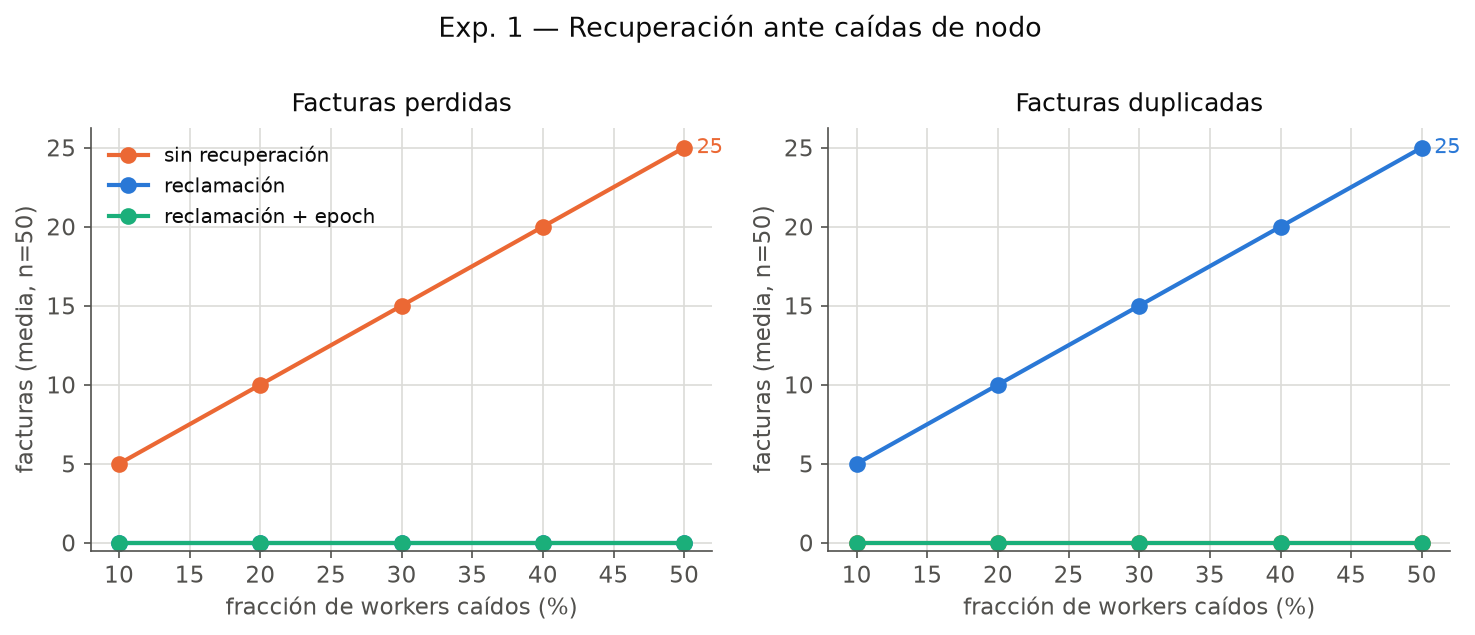
\includegraphics[width=\linewidth]{figuras/exp1_recuperacion.png}
\caption{Facturas perdidas (izq.) y duplicadas (der.) frente a la fracción de workers
caídos. \texttt{none} pierde linealmente; \texttt{reclaim} recupera pero duplica;
\texttt{reclaim+epoch} queda en cero en ambos paneles.}
\end{figure}

\hallazgo{Sin recuperación, las pérdidas crecen linealmente con la fracción de caídas (de 5 a
25 facturas, 10\,\%$\to$50\,\%). La reclamación las elimina (0), pero cada worker zombi que
resucita pisa el record bueno $\Rightarrow$ tantas facturas duplicadas/corruptas como caídas.
El \emph{epoch fencing} elimina también los duplicados (los 15 zombis son rechazados) y es el
\emph{único} modo cuyo resultado final coincide bit a bit con una corrida sin fallos. El
desvío entre semillas es 0: la recuperación es determinista por diseño.}

\subsection{Experimento 2 — Corrupción silenciosa y alucinación}

Sobre facturas reconstruidas correctamente se inyectan errores controlados (25\,\%
corrupción, 25\,\% alucinación) y se compara \emph{con} y \emph{sin} VERA.

\begin{table}[h]
\centering\small
\begin{tabular}{@{}l l ccc cc@{}}
\toprule
\textbf{Corpus} & \textbf{Condición} & \textbf{Detección} & \textbf{FP} & \textbf{FN} &
\textbf{Det.\ corrup.} & \textbf{Det.\ alucin.} \\
\midrule
sintético (100) & \textbf{con VERA} & \textbf{1.00} & 0 & 0 & 1.00 & 1.00 \\
sintético (100) & sin VERA & 0.00 & 0 & \textbf{50} & 0.00 & 0.00 \\
real (${\sim}50$) & \textbf{con VERA} & \textbf{1.00} & 0 & 0 & 1.00 & 1.00 \\
real (${\sim}50$) & sin VERA & 0.00 & 0 & \textbf{24} & 0.00 & 0.00 \\
\bottomrule
\end{tabular}
\caption{Detección por corpus y condición (media de 10 semillas; desvío $=0$). FP: falsos
positivos (buenas rechazadas); FN: falsos negativos (malas que entran al PDF).}
\end{table}

\begin{figure}[h]
\centering
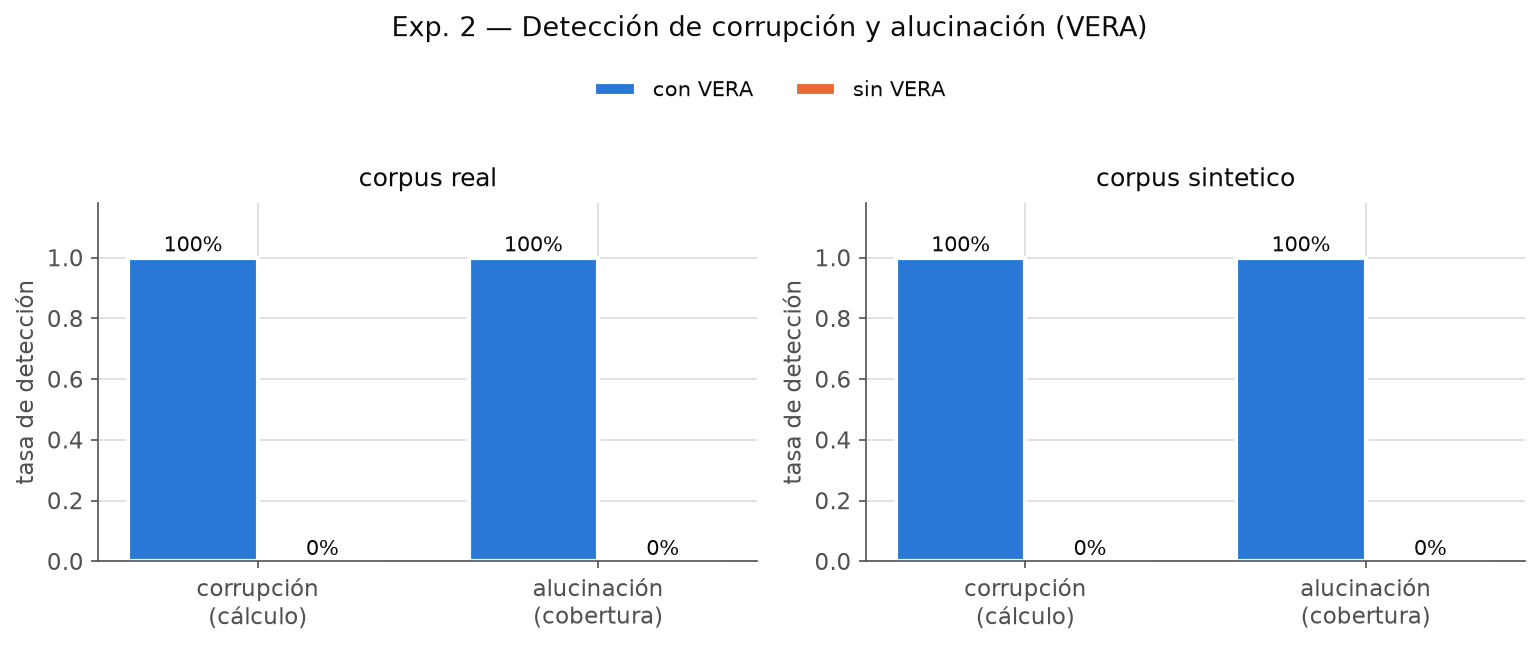
\includegraphics[width=\linewidth]{figuras/exp2_deteccion.png}
\caption{Tasa de detección por tipo de fallo, con y sin VERA, en ambos corpus. La corrupción
la caza la dimensión de cálculo; la alucinación, la de cobertura. Sin VERA no se detecta
nada.}
\end{figure}

\begin{figure}[h]
\centering
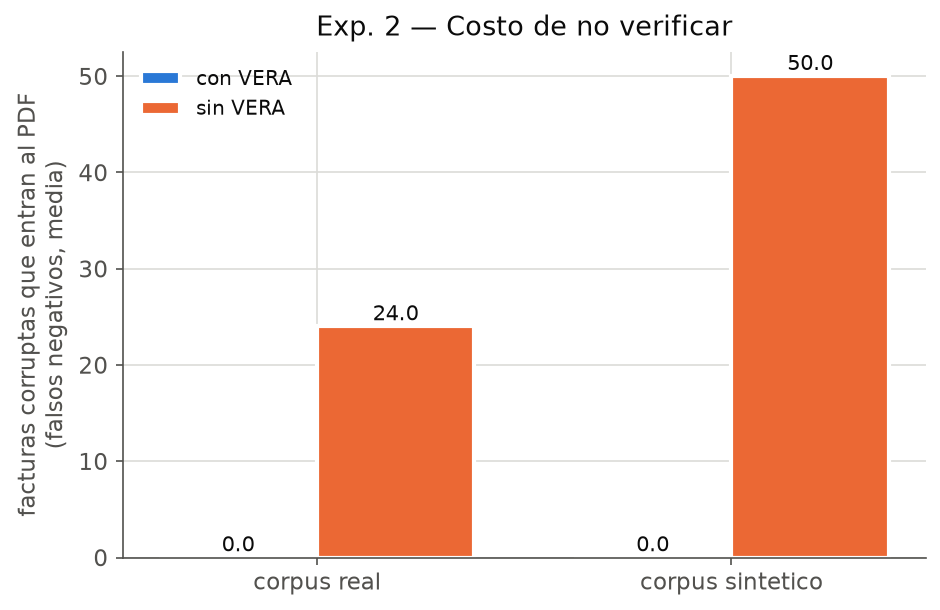
\includegraphics[width=0.72\linewidth]{figuras/exp2_falsos_negativos.png}
\caption{Costo de no verificar: sin VERA, 24 (real) y 50 (sintético) facturas corruptas
entran al PDF; con VERA, ninguna.}
\end{figure}

\hallazgo{Con VERA la detección es perfecta (100\,\%) en ambos fallos, con cero falsos
positivos y negativos, tanto en el corpus sintético como en el de facturas \emph{reales}. Sin
VERA, ninguna corrupción se detecta: 24--50 facturas con datos inventados o inconsistentes
entran al PDF. Cada fallo lo caza una dimensión distinta de VERA; las dos son necesarias.}

% ===========================================================================
\section{Fortalecimiento experimental: reconstrucción real y verificación independiente}
\label{sec:fort}

Los resultados de §\ref{sec:res} usan un reconstructor \emph{oracle} y verifican VERA contra
una fuente \textbf{privilegiada} (el texto limpio, derivado de la verdad). Son un \emph{techo}
útil, pero con dos circularidades. Esta sección las levanta: reconstructor \textbf{real} y
fuente de verificación \textbf{independiente}. Conviene separar tres niveles de garantía:
\textbf{(A)}~ejecución, \textbf{(B)}~calidad de reconstrucción, \textbf{(C)}~verificación.

\paragraph{(A) Garantías de ejecución.} El commit valida el \emph{epoch} contra el estado
\textbf{durable} (disco), no una caché, dentro de un lock de fichero (\texttt{flock}) que
serializa a todos los procesos: la comprobación del token y la escritura son una sola
operación atómica, sin TOCTOU entre procesos (probado con dos procesos reales). La
denominación correcta de la garantía es \textbf{at-least-once execution} (un intento caído se
re-ejecuta) con \textbf{exactly-once effect} (commits idempotentes con epoch fencing: un record
por factura, el de mayor epoch; los zombis se rechazan). \emph{No} es exactly-once
\emph{processing}: el trabajo de reconstrucción puede repetirse.

\paragraph{(B) Calidad de reconstrucción.} Se definieron tres modos con interfaz común; los
productivos \textbf{no} acceden a la verdad (verificado por test). \textsc{Oracle} (baseline),
\textsc{Conservador} (conserva lo legible, abstiene lo ilegible) y \textsc{LLM-GSR} real
(backend local \texttt{qwen3.5:35b} vía Ollama; OpenAI \texttt{gpt-4o} quedó bloqueado por
límite de gasto). El gold se compara \emph{solo} en el evaluador.

\begin{table}[h]
\centering\small
\begin{tabular}{@{}l l ccccc@{}}
\toprule
\textbf{OCR} & \textbf{Modo} & \textbf{Exac.\ campo} & \textbf{Exac.\ si resp.} &
\textbf{Fact.\ exacta} & \textbf{Alucinación} & \textbf{Abstención} \\
\midrule
clean    & conservador & 0.911 & 0.981 & 0.50  & 0.018 & 0.071 \\
clean    & \textbf{llm} & 0.982 & 0.982 & 0.875 & 0.018 & 0.00 \\
degraded & conservador & 0.696 & 0.951 & 0.125 & 0.036 & 0.268 \\
degraded & \textbf{llm} & 0.893 & 0.909 & 0.375 & 0.089 & 0.018 \\
poor     & conservador & 0.554 & 0.838 & 0.00  & 0.107 & 0.339 \\
poor     & \textbf{llm} & 0.786 & 0.830 & 0.125 & 0.161 & 0.054 \\
\bottomrule
\end{tabular}
\caption{Calidad de reconstrucción por grado de degradación ($n=8$/grado; oracle $=1.0$ por
construcción). El LLM recupera más que el conservador, pero \textbf{alucina más} al degradarse
el OCR (0.018$\to$0.089$\to$0.161), mientras el conservador \textbf{abstiene} más
(0.07$\to$0.27$\to$0.34): los dos regímenes de la Precondición de Reconstrucción.}
\end{table}

\paragraph{(C) Garantías de verificación.} Se estresó a VERA con \textbf{diez familias de
fallos adversariales} (importe inventado pero aritméticamente consistente, CUIT válido
incorrecto, valor de otro documento, línea omitida/sustituida, campo con evidencia degradada,
etc.) más facturas limpias, con gate estricto (REVIEW/UNVERIFIED en campo requerido
\emph{no} pasa).

\begin{table}[h]
\centering\small
\begin{tabular}{@{}l l cccc@{}}
\toprule
\textbf{Fuente} & \textbf{Dimensiones} & \textbf{Recall} & \textbf{FRR} & \textbf{Precisión} & \textbf{F1} \\
\midrule
privilegiada (texto limpio) & cobertura+cálculo & 1.00 & 0.00 & 1.00 & 1.00 \\
privilegiada & solo cálculo & 0.432 & 0.00 & 1.00 & 0.603 \\
\textbf{independiente} (OCR degradado) & cobertura+cálculo & 1.00 & \textbf{0.897} & 0.698 & 0.822 \\
\textbf{independiente} & solo cálculo & 0.432 & \textbf{0.00} & 1.00 & 0.603 \\
\bottomrule
\end{tabular}
\caption{VERA frente a 10 fallos adversariales (120 casos; IC95 de Wilson para recall
$=[0.955,1.0]$). FRR: tasa de falso rechazo (limpias rechazadas).}
\end{table}

\hallazgo{El 100\,\%/0\,FP de §\ref{sec:res} \textbf{solo se sostiene con la fuente
privilegiada}: es una circularidad (VERA termina comparando contra algo derivado de la verdad).
Con una fuente \emph{independiente} (el OCR degradado que vio el reconstructor), la
\textbf{cobertura deja de ser una compuerta dura} ---rechaza casi todas las limpias (FRR
0.90) porque el ruido impide anclar incluso valores correctos--- y queda como señal de
\emph{revisar}. El \textbf{cálculo} es la dimensión robusta e independiente de la fuente (FRR 0,
precisión 1.0) pero \textbf{no generaliza}: recall 0.43, solo caza rupturas aritméticas.}

\paragraph{Abstención y calibración.} Un criterio de abstención por evidencia+confianza es, en
principio, la defensa contra la alucinación. Pero al barrer el umbral de confianza $\tau$ sobre
el LLM, el riesgo (error entre respondidos) baja apenas de 0.108 a 0.083 y la cobertura casi no
cae: \texttt{qwen3.5:35b} reporta confianza \textbf{uniformemente alta} aun cuando se equivoca
---está \textbf{mal calibrado}---, de modo que su autoconfianza no separa aciertos de errores.
La abstención \emph{estructural} por evidencia (la del modo conservador) resulta la palanca
honesta efectiva. Sobre $I(\hat c;s)$: es una cantidad \emph{poblacional}; no se mide por
documento (no hay estimador insesgado de un solo par), por lo que la recuperabilidad se reporta
\emph{empíricamente} a nivel corpus (tabla de calidad), no como un falso ``IM por factura''.

% ===========================================================================
\section{Discusión y limitaciones}

Los resultados cuantifican la tesis: \emph{lease} + \emph{epoch fencing} logran un
\textbf{efecto} exactamente-una-vez (0 pérdidas, 0 duplicadas en el resultado; la ejecución en
sí sigue siendo at-least-once, §\ref{sec:fort}), pero eso \textbf{no} basta para
la correctitud; sin la compuerta VERA, decenas de facturas corruptas entran al PDF sin que el
sistema lo note. Las dos preguntas ---¿se perdió trabajo? y ¿es correcto el contenido?--- son
ortogonales y hace falta un mecanismo para cada una.

Es honesto declarar las simplificaciones del montaje:
\begin{itemize}[leftmargin=1.4em,itemsep=1pt]
  \item \textbf{Reconstructor determinista en la parte A.} Los experimentos de recuperación
    usan el \emph{oracle} (temperatura 0, verdad) para que el ruido OCR no interfiera en la
    medición de la \emph{recuperación} y la \emph{compuerta}. La §\ref{sec:fort} levanta esta
    simplificación con un reconstructor \textbf{real} (LLM-GSR) y mide su calidad frente al OCR
    degradado.
  \item \textbf{Desvío cero.} Los resultados son robustos, pero porque el modelo de
    recuperación es determinista, no por muestreo estadístico sobre corridas estocásticas.
  \item \textbf{Detección 100\,\%.} VERA atrapa todo porque los errores inyectados caen dentro
    de la cobertura de sus reglas por construcción. Alucinaciones reales de un LLM pueden caer
    fuera de esa cobertura; VERA solo detecta lo que sus reglas cubren.
  \item \textbf{Caídas simuladas en un nodo} (reloj virtual determinista), no en red real; el
    corpus es de un solo dominio (facturas).
\end{itemize}

% ===========================================================================
\section{Conclusión}

Se construyó y evaluó un pipeline distribuido de reconstrucción de facturas con recuperación
ante fallos y una compuerta de verificación. La arquitectura de \emph{lease} con reclamación
y \emph{epoch fencing} elimina pérdidas y duplicados ante caídas de nodo, y reproduce bit a
bit el resultado de una corrida sin fallos. La compuerta VERA, con sus dimensiones de
cobertura y cálculo, detecta los fallos inyectados; pero ese 100\,\% \textbf{depende de la
fuente}: solo se sostiene contra el texto limpio privilegiado. Con una fuente independiente
(§\ref{sec:fort}), el recall se mantiene pero la cobertura deja de ser compuerta dura (falsos
rechazos altos) y el cálculo ---robusto--- caza solo rupturas aritméticas. El trabajo deja
cuantificada la idea que lo guía: \emph{procesar cada factura exactamente una vez no garantiza
que el resultado sea correcto}; y, de forma honesta, también el límite de la propia
verificación.

% ===========================================================================
\appendix
\section{Reproducibilidad}

Código en el repositorio del trabajo. Entorno: Python 3.11 (venv limpio \texttt{.venv311};
el \texttt{.venv} del proyecto hereda ROS y contamina \texttt{PYTHONPATH}).

\begin{lstlisting}[language=bash]
# instalar
python3.11 -m venv .venv311 && .venv311/bin/pip install -r requirements.txt

# prefijo (neutraliza el entorno ROS)
RUN="env -u PYTHONPATH PYTHONNOUSERSITE=1 .venv311/bin/python"

$RUN run.py exp1 --real        # caidas de nodo (3 modos), facturas reales
$RUN run.py exp2 --real        # corrupcion + alucinacion, con/sin VERA

# parte B (fortalecimiento)
$RUN -m experiments.exp2_real            # calidad Oracle/Conservador/LLM-GSR (usa LLM)
$RUN -m experiments.exp3_vera_adversarial # VERA vs 10 fallos adversariales
$RUN -m experiments.exp4_abstention       # abstencion vs reconstruir siempre

# tests
env -u PYTHONPATH PYTEST_DISABLE_PLUGIN_AUTOLOAD=1 PYTHONNOUSERSITE=1 \
    .venv311/bin/python -m pytest framework/vera/tests tests -q   # 385 passed, 1 skipped
\end{lstlisting}

\paragraph{Componentes.} \texttt{pipeline/}: \texttt{leases} (recuperación), \texttt{store} /
\texttt{redis\_store} (epoch fencing en disco / Redis), \texttt{gate} (compuerta VERA de dos
dimensiones), \texttt{reconstructor} (tres modos: oracle, conservador y LLM-GSR real), \texttt{faults} (inyección),
\texttt{orchestrator} / \texttt{ray\_dispatcher} (ejecutores), \texttt{real\_corpus} (facturas
reales), \texttt{pdf}. \texttt{framework/vera/}: el verificador. \texttt{experiments/}: los
experimentos (recuperación, compuerta y fortalecimiento) y el arnés de medición.
